\suppnote{Held-out coupling and baseline results}{note:coupling-results}

\begin{table}[!htbp]
\centering\footnotesize
\caption{\textbf{Three-city P/D/CLIM scores.} P scores the raw target; D scores TRAIN-centred departures; CLIM is the source-free P/ROAD phase clock. Cov.\ is raw routing energy captured by roads. Errors pool held-out observations within each city.}
\label{tab:crosscity}
\setlength{\tabcolsep}{3pt}
\begin{tabular*}{\textwidth}{@{\extracolsep{\fill}}lrrrrrrrrr@{}}
\toprule
 & & & \multicolumn{4}{c}{P} & \multicolumn{3}{c}{D} \\
\cmidrule(lr){4-7}\cmidrule(lr){8-10}
City & Cov. & CLIM & \multicolumn{2}{c}{UrbanFlow} & Ridge & POD & \multicolumn{2}{c}{UrbanFlow} & Ridge \\
\cmidrule(lr){4-5}\cmidrule(lr){8-9}
 & & ROAD & ROAD & FACE & FACE & FACE & ROAD & FACE & FACE \\
\midrule
Porto & 0.904 & 0.472 & 0.682 & 0.607 & 0.701 & 0.701 & 0.468 & 0.411 & 0.504 \\
San Francisco & 0.886 & 0.727 & 0.597 & 0.528 & 0.611 & 0.637 & 0.240 & 0.209 & 0.262 \\
Chengdu & 0.731 & 0.931 & 0.606 & 0.440 & 0.572 & 0.575 & 0.120 & 0.085 & 0.126 \\
\bottomrule
\end{tabular*}
\end{table}

The three focal cities replicate a procedure, not a single operator transferred between cities. Porto has the strongest departure coupling. San Francisco retains positive D scores despite a raw climatology stronger than raw operator reconstruction. Chengdu separates a highly recurrent raw field from weak departure prediction: P/ROAD is 0.606, CLIM is 0.931 and D/ROAD is 0.120. Adding the D departure to the TRAIN climatology gives a full-field gain $\Delta R_I=(1-R_{\rm CLIM})R_D$ of approximately 0.25, 0.07 and 0.008 in Porto, San Francisco and Chengdu. The evidence is therefore hierarchical rather than three equivalent validations: Porto shows a clear conditional relation, San Francisco a weaker but consistent one, and Chengdu a highly recurrent field in which source information adds little beyond the daily pattern.

Paired-date bootstrap intervals for D/ROAD are 0.355--0.528 in Porto, 0.188--0.288 in San Francisco and 0.107--0.142 in Chengdu (10,000 resamples, dates resampled within folds). The source--routing pairing null permutes complete date blocks within TRAIN, VAL and TEST separately and refits the operator in each of 199 draws; null medians are approximately zero, and no Porto or San Francisco draw reaches the observed score (empirical $p=1/200$). Chengdu has only three held-out dates, so its null and interval are descriptive rather than significance tests. Figure~\ref{fig:supp-2} shows the date-resolved values.

Full-face ridge and TRAIN-only POD equal or outperform the road restriction on FACE targets. D/FACE ridge scores are 0.504, 0.262 and 0.126, against road-restricted 0.411, 0.209 and 0.085. Roads therefore supply independently specified, interpretable support rather than the highest linear reconstruction accuracy. Interior-face counts in Porto, San Francisco and Chengdu are 1,984, 5,512 and 7,080; D-frame selected POD ranks are 958, 16 and 64. Table~\ref{tab:crosscity} consistently pools errors rather than averaging fold scores.

\paragraph{Three-city P-frame physical reconstruction.} Figure~\ref{fig:supp-6} visualizes observed and predicted road-supported routing fields using the frozen P estimator with raw TEST inputs and targets. No phase climatology is added and no D departure is substituted. Porto and San Francisco preserve their archived \texttt{picked\_i}/\texttt{picked\_phase} snapshots. Chengdu selects the TEST date whose daily P error is closest to the median daily P error: \texttt{picked\_i=2}, \texttt{picked\_phase=6} (12:00 in the 06--23\,h window), \texttt{picked\_date=16304}. Its pinned-basis export is checked against the frozen $R_{\mathrm P}$. These snapshots are qualitative complements to the complete pooled scores, not additional independent experiments.

\begin{figure}[!htbp]
\centering
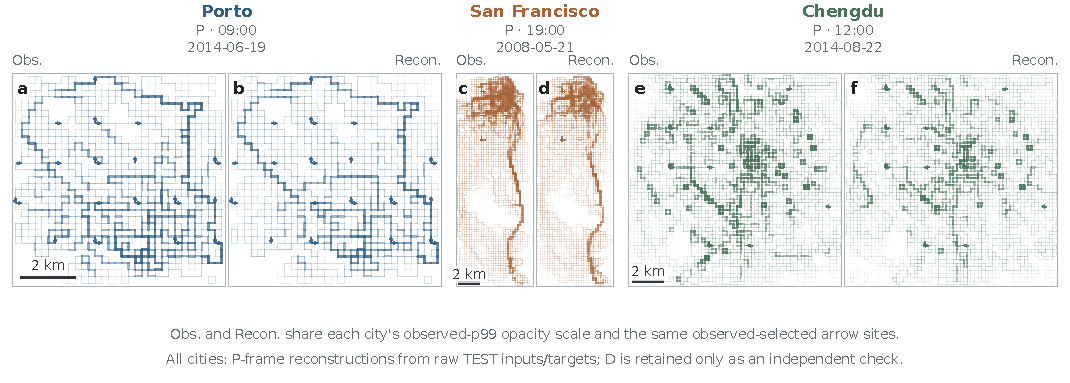
\includegraphics[width=\textwidth]{figS06_heldout_reconstruction.pdf}
\caption{\textbf{Three-city held-out physical reconstruction in the P frame.} Observed and reconstructed road-supported routing fields for Porto, San Francisco and Chengdu, using the frozen P estimator with raw TEST inputs and targets; no phase climatology is added. Porto and San Francisco preserve their archived picked indices and phases. Chengdu uses the TEST date with daily P error closest to the median daily P error, specifically \texttt{picked\_i=2}, \texttt{picked\_phase=6} (12:00), \texttt{picked\_date=16304}, and passes the pinned-basis/frozen-$R_{\mathrm P}$ export check. Observed and predicted panels within a city use identical glyph sites and the observed field's 99th-percentile magnitude scale, with saturation above it; colour scales are city-specific. The maps are qualitative, whereas Table~\ref{tab:crosscity} uses every held-out observation.}
\label{fig:supp-6}
\end{figure}

\paragraph{Neural aggregation.} Seed configuration variability, the archived Porto paired contrast and the sealed seed means are reported in Note~\ref{note:baselines}. Table~\ref{tab:crosscity} and main Table~1 use archived pooled per-date errors, including a San Francisco Graph WaveNet value pooled from its archived per-date records; the sealed San Francisco fold mean is not used for ranking.

\paragraph{Gravity and loading diagnostics.} Native gravity CPC values are 0.525, 0.464 and 0.555. TEST-scaled gravity loading gives 0.136, 0.270 and $8.3\times10^{-5}$; exact-TEST-OD AON gives 0.172, 0.336 and 0.002, with fixed-amplitude values 0.126, $-0.533$ and $-0.565$. These tasks use different inputs and are not source-only accuracy rankings.

Chengdu's OD table contains 1.64\,M TEST trips, of which 1.28\,M remain after snapping. Its strong OD overlap but near-zero loading score is therefore not a ranking of demand quality. The loaded field has cosine 0.04 with the observed field, and destination permutation leaves the loaded field almost unchanged (cosine 0.93--0.94), showing that this pipeline resolves a largely margin-driven pattern. Rebuilding the observed three TEST dates from all fixes reproduces the frozen field at pooled cosine 0.999999. Using occupied runs alone removes 16.3\% of absolute flux, leaves 76\% of energy, and gives pooled cosine 0.929 with the all-fix field. Thus the activity-set difference is real and bounded, but by itself is unlikely to account for the loading mismatch. All loading rows diagnose the implemented demand--registration--loading pipeline rather than attainable performance of traffic assignment as a paradigm.
